\documentclass[9pt,pdf,utf8,hyperref={unicode},aspectratio=169]{beamer}

%Привычный шрифт для математических формул
\usefonttheme[onlymath]{serif}
\mode<presentation>
{
    \usetheme{boxes}
    \beamertemplatenavigationsymbolsempty

    \setbeamercovered{transparent}
    \setbeamertemplate{navigation symbols}{}
    
    \setbeamertemplate{footline}[frame number]
    \setbeamertemplate{caption}[numbered]
    % \setbeamersize{text margin left=0.5em, text margin right=0.5em}
}

% Дополнительные библиотеки
\usepackage[T2A]{fontenc}
\usepackage[english, russian]{babel}
\usepackage[utf8]{inputenc}
\usepackage{amsmath,amssymb}
\usepackage{indentfirst}
\usepackage{changepage}
\usepackage{enumerate}
\usepackage{mathtools}
\usepackage{multicol}
\usepackage{multirow}
\usepackage{ragged2e}
\usepackage{multicol}
\usepackage{diagbox}
\usepackage{wrapfig}
\usepackage{comment}
\usepackage{subfig}
\usepackage{array}
\usepackage{color}
\usepackage{tikz}
\usepackage{url}
\usepackage{bm}

\usetikzlibrary{trees}

% Определение дополнительных функций
\DeclareMathOperator*{\plim}{\mathop{plim}}
\DeclareMathOperator{\prob}{\mathbf{P}\!}

\DeclareMathOperator{\arctanh}{arctanh}
\DeclareMathOperator{\mmode}{mode}
\DeclareMathOperator{\rank}{rank}
\DeclareMathOperator{\diag}{diag}
\DeclareMathOperator{\sign}{sign}
\DeclareMathOperator{\cov}{cov}
\DeclareMathOperator{\pow}{pow}
\DeclareMathOperator{\med}{med}

\def\argmin#1{ \mathop{\text{argmin}}\limits_{#1} }
\def\argmax#1{ \mathop{\text{argmax}}\limits_{#1} }

\newcommand{\tsum}{\mathop{\textstyle\sum}\limits}
\newcommand{\condprob}[2] {\mathbf{P}\!\left(#1\left|#2\right.\right)}

\renewcommand{\leq}{\leqslant}
\renewcommand{\geq}{\geqslant}

\DeclareMathOperator{\FWER}{FWER}
\DeclareMathOperator{\FDR}{FDR}
\newtheorem{Th}{Теорема}
\newtheorem{Def}{Определение}

% Основная часть

\title[Причинность]{Прикладной статистический анализ данных\\Причинно-следственные связи}
\author{Андрей Грабовой}
\date{}

\begin{document}
\tikzstyle{every node}=[draw=black,thick,anchor=west]
\tikzstyle{selected}=[draw=red,fill=red!30]
\tikzstyle{optional}=[dashed,fill=gray!50]

\begin{frame}
    \titlepage
\end{frame}

\section{Причинность и графы}
\subsection{Парадокс Симпсона}
\begin{frame}{Исследование уровня холестерина}
	\only<1>{
		\begin{center}
			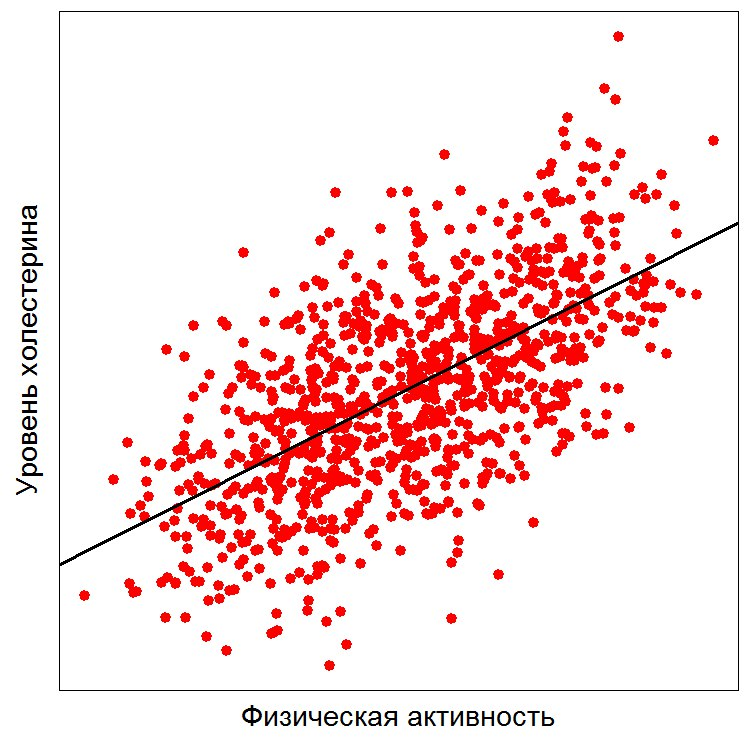
\includegraphics[width=0.55\linewidth]{imgs/cholesterol}
		\end{center}
	}
	\only<2>{
		\begin{center}
			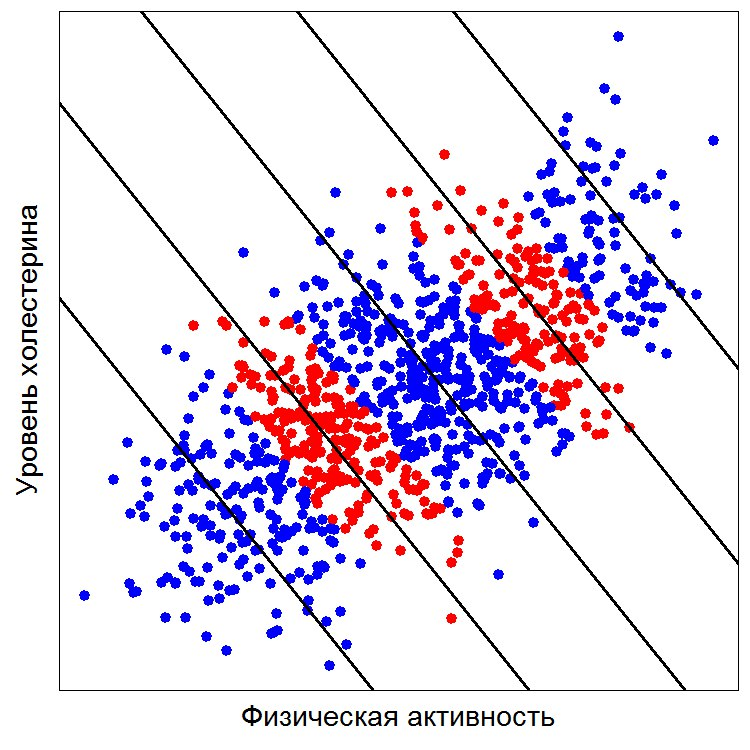
\includegraphics[width=0.55\linewidth]{imgs/cholesterol_level}
		\end{center}
    }
\end{frame}


\begin{frame}{Парадокс Симпсона}
\only<1>{
Пример 1:

  \begin{tabular}{|c|c|c|c}
	\cline{1-3}
	$\Sigma$ & лекарство & плацебо & \\
	\cline{1-3} 
	выздоровели & 273 & 289 & плацебо на 5\%\\
	\cline{1-3}
	не выздоровели & 77 & 61 & эффективнее \\
	\cline{1-3}
	 & 78\% & 83\% & \\
	\cline{1-3}
\end{tabular} \\
$ $ \\
$ $ \\
  \begin{tabular}{|c|c|c|c}
	\cline{1-3}
    \textbf{мужчины} & лекарство & плацебо &\\
	\cline{1-3}
	выздоровели & 81 & 234 & лекарство на 5\% \\
	\cline{1-3}
	не выздоровели & 6 & 36 & эффективнее \\
	\cline{1-3}
	 & 93\% & 87\% & \\
	\cline{1-3}
\end{tabular} \\
$ $ \\
$ $ \\
  \begin{tabular}{|c|c|c|c}
	\cline{1-3}
	\textbf{женщины} & лекарство & плацебо\\
	\cline{1-3}
	выздоровели & 192 & 55 & лекарство на 4\% \\
	\cline{1-3}
	не выздоровели & 71 & 25 & эффективнее \\
	\cline{1-3}
	 & 73\% & 69\% \\
	\cline{1-3}
\end{tabular}
}

\only<2>{
	Какой из двух выводов верен? 
	
	\bigskip
	
	Предположение: верны выводы по отдельным подгруппам, потому что они основаны на более детальной информации.
	
	\bigskip
	
	Это предположение неверно — всё зависит от того, как признак, по которому происходит разбиение на подгруппы, связан с остальными анализируемыми признаками.
}

\only<3>{
Пример 2:

  \begin{tabular}{|c|c|c|c}
	\cline{1-3}
	$\Sigma$ & лекарство & плацебо & \\
	\cline{1-3} 
	выздоровели & 273 & 289 & плацебо на 5\%\\
	\cline{1-3}
	не выздоровели & 77 & 61 & эффективнее \\
	\cline{1-3}
	 & 78\% & 83\% & \\
	\cline{1-3}
\end{tabular} \\
$ $ \\
$ $ \\
  \begin{tabular}{|c|c|c|c}
	\cline{1-3}
    \begin{tabular}{@{}c@{}}\textbf{низкое давление} \\ \textbf{в конце лечения} \end{tabular} & лекарство & плацебо &\\
	\cline{1-3}
	выздоровели & 81 & 234 & лекарство на 5\% \\
	\cline{1-3}
	не выздоровели & 6 & 36 & эффективнее \\
	\cline{1-3}
	 & 93\% & 87\% & \\
	\cline{1-3}
\end{tabular} \\
$ $ \\
$ $ \\
  \begin{tabular}{|c|c|c|c}
	\cline{1-3}
	\begin{tabular}{@{}c@{}}\textbf{низкое давление} \\ \textbf{в конце лечения} \end{tabular} & лекарство & плацебо\\
	\cline{1-3}
	выздоровели & 192 & 55 & лекарство на 4\% \\
	\cline{1-3}
	не выздоровели & 71 & 25 & эффективнее \\
	\cline{1-3}
	 & 73\% & 69\% \\
	\cline{1-3}
\end{tabular}
}
\end{frame}

\subsection{Причинные графы}
\begin{frame}{Причинные графы}
Отношения причинности могут быть представлены в виде направленного графа, вершины которого соответствуют признакам, а наличие пути говорит о существовании причинно-следственной связи. 

\bigskip

\textbf{Путь} — последовательность вершин, где каждая вершина соединена со следующей ребром. 
    
    
\textbf{Направленный путь} — путь, в котором все ребра имеют одинаковое направление.


\textbf{Путь через заднюю дверь (ПЗД)} от $X$ к $Y$ — такой путь, который начинается с $X \leftarrow$, а заканчивается $\rightarrow Y$. 
\end{frame}

\begin{frame}{Элементы причинного графа}
\only<1>{
\begin{center}
	$X \rightarrow Y \rightarrow Z $ — \textbf{цепочка}
\end{center}

Пример:
\begin{itemize}
	\item $X$~--- бюджет школы
	\item $Y$~--- средний балл учеников
	\item $Z$~--- доля поступающих в ВУЗы
\end{itemize}

\bigskip
Свойства:
\begin{enumerate}
    \item $X$ и $Y$, $Y$ и $Z$ — зависимы: \\
    $\exists x, y: \condprob{Y = y}{X = x} \neq \prob\left(Y = y\right) $ \\
    $\exists y, z: \condprob{Z = z}{Y = y} \neq \prob\left(Z = z\right) $
    \item $Z$ и $X$ — скорее всего, зависимы  
    \item $Z\perp X | Y$ — условно независимы: $\forall x, y, z$ $$\condprob{Z = z}{X=x, Y = y} = \condprob{Z = z}{Y = y}$$ (если $Y$ фиксировано, то $X$ и $Z$ независимы)
\end{enumerate}
}
\only<2>{

\begin{center}
	$Y \leftarrow X \rightarrow Z $ — \textbf{вилка}
\end{center} 


Пример: 
\begin{itemize}
	\item $X$~--- продажи мороженого
	\item $Y$~--- средняя дневная температура воздуха
	\item $Z$~--- число преступлений
\end{itemize}


\bigskip
Свойства:
\begin{enumerate}
    \item $X$ и $Y$, $X$ и $Z$ — зависимы
    \item $Y$ и $Z$ —  скорее всего, зависимы  
    \item $Y$ $\perp$ $Z | X$ — условно независимы
\end{enumerate}
}

\only<3>{

\begin{center}
	$Y \rightarrow X \leftarrow Z $ — \textbf{коллайдер}
\end{center} 

\bigskip
	


Пример (парадокс Монти-Холла):
\begin{itemize}
	\item $X$~--- выбор ведущего
	\item $Y$~--- выбор игрока
	\item $Z$~--- положение приза
\end{itemize}



\bigskip

Свойства:
\begin{enumerate}
    \item $Y$ и $X$, $Z$ и $X$ — зависимы\\
    \item $Y$ и $Z$ — независимы
    \item $Y$ $\not \perp$ $Z | X$ — условно зависимы
\end{enumerate}
}
\end{frame}

\begin{frame}{d-разделимость}
\only<1>{
Путь $P$ \textbf{блокируется} переменной $Z$, если: 
\begin{enumerate}
    \item $P$ содержит $A \rightarrow B \rightarrow C$,
    $A \leftarrow B \rightarrow C$, $B \in Z$
    \item $P$ содержит $A \rightarrow B \leftarrow C$, $B \notin Z$ и все потомки $B \notin Z$ 
\end{enumerate}

\bigskip

Если $Z$ блокирует все пути из $X$ в $Y$, то $X$ и $Y$ \textbf{d-разделимы}.
}
\only<2->{
Пример:
\begin{center}
	\begin{tikzpicture}
	    \node at (0,2) (z1) {$Z_1$};<br>
	    \node at (4,2) (z2) {$Z_2$}; <br>
	    \node at (2,1) (z3) {$Z_3$};<br>
	    \node at (0,0) (x) {$X$};<br>
	    \node at (4,0) (y) {$Y$};<br>
	    \node at (2,0) (w) {$W$};<br>
	    <br>
	    \path[->] (z1) edge (x) ;<br>
	    \path[->] (z1) edge (z3);<br>
	    \path[->] (z2) edge (z3) ;<br>
        \path[->] (z2) edge (y) ;<br>
        \path[->] (z3) edge (x) ;<br>
        \path[->] (z3) edge (y) ;<br>
        \path[->] (x) edge (w) ;<br>
        \path[->] (w) edge (y) ;<br>
	\end{tikzpicture}
	
	\bigskip
	
	\begin{tabular}{|c|c|}\hline
	Упорядоченная пара вершин & d-разделяющее множество \\ \hline
	$(Z_1, W)$ & $X$ \\
	$(Z_1, Y)$ & \uncover<3->{$\{Z_3, X, Z_2\}, \{Z_3, W, Z_2\}$ } \\
	$(X, Y)$ & \uncover<3->{$\left\{W, Z_3, Z_1\right\}$} \\\hline
	\end{tabular}
\end{center}
}
\end{frame}




\section{Восстановление графа}

\subsection{Восстановление графа по статическим данным}
\begin{frame}{Алгоритм индуктивной причинности}
\only<1>{
	Вход: множество вершин $V$
	\begin{enumerate}
	\item $\forall A,B \in V$ ищем множество $S_{AB} \colon  A \perp B | S_{AB}, \; A,B\notin S_{AB}.$ Если такого $S_{AB}$ не существует, соединяем $A$ и $B$ ребром.
	\item $\forall A,B,$ не связанных ребром и имеющих общего соседа $C$, проверяем: $C\in S_{AB}$? Если нет, то заменяем пару рёбер $A-C, C-B$ на пару ориентированных рёбер $A\rightarrow C, C\leftarrow B$
	\item Рекурсивно применяем следующие два правила:
		\begin{itemize}
		\item если из $A$ в $B$ есть ориентированный путь $A\rightarrow\dots\rightarrow B$, то $A-B$ заменяем на $A\rightarrow B$;
		\item если $A$ и $B$ не соединены, $A\rightarrow C$, $C-B$, то $C-B$ заменяем на $C\rightarrow B$.
		\end{itemize}
	\end{enumerate}
	Выход: ориентированный (возможно, частично) граф $G$. 
	}
\only<2>{
	Правила (1) и (2) применять в чистом виде невозможно — числи перебираемых множеств экспоненциально растёт с числом вершин графа. Поэтому используются сокращающие перебор эвристики.
	
	\bigskip
	
	\begin{center}
	\begin{tabular}{|p{3cm}|p{3.5cm}|p{3.5cm}|}\hline
	Признаки & дискретные & непрерывные \\\hline
	Распределение & мультиномиальное & нормальное \\\hline
	Критерий условной независимости & хи-квадрат для трёхмерных таблиц сопряжённости & Стьюдента для частной корреляции \\\hline
	Критерий качества графа & \multicolumn{2}{c|}{$BIC$} \\\hline
	\end{tabular}
	\end{center}
}
\end{frame}


\subsection{Восстановление графа по динамическим данным}
\begin{frame}{Причинность по Грейнджеру}
    Между рядами $x_1,\dots,x_T$ и $y_1,\dots,y_T$ существует \textbf{причинная связь Грейнджера $x_t \rightarrow y_t$}, если дисперсия ошибки оптимального прогноза $\hat{y}_{t+1}$ по $y_1,\dots,y_t,x_1,\dots,x_t$ меньше, чем только по $y_1,\dots,y_t$.

    \bigskip

Причинность по Грейнджеру
\begin{itemize}
	\item может следовать из причинно-следственной связи;
	\item не является достаточным условием причинно-следственной связи.
\end{itemize}
     
    \bigskip

    $x_1,\dots,x_T$ и $y_1,\dots,y_T$ \textbf{взаимосвязаны}, если $x_t \rightarrow y_t$ и $y_t \rightarrow x_t$.
\end{frame}

\begin{frame}{Критерий Грейнджера}
    \only<1>{
    \vspace{-12pt}
    $$y_t = \alpha + \sum_{i=1}^{k_1} \phi_{1i} y_{t-i} + \sum_{i=1}^{k_2} \phi_{2i} x_{t-i} + \varepsilon_t.$$
    $k_1$ и $k_2$ выбирается по информационному критерию.
    $$x_t \rightarrow y_t \;\; \Rightarrow \;\; \exists \phi_{2i}\neq 0.$$
  \begin{center}
        \begin{tabular}{rl}
            нулевая гипотеза:               & $H_0\colon \phi_{21}=\dots=\phi_{2k_2}=0;$ \\
            альтернатива:                   & $H_1\colon H_0$ неверна;\\
            статистика:                     & $F = \frac{\left(RSS_{r}-RSS_{ur}\right) / k_2} {RSS_{ur} / \left(T-k_1-k_2-1\right)};$ \\
                                            & $F \sim F(k_1,T-k_1-k_2-1)$ при $H_0.$\\
        \end{tabular}
        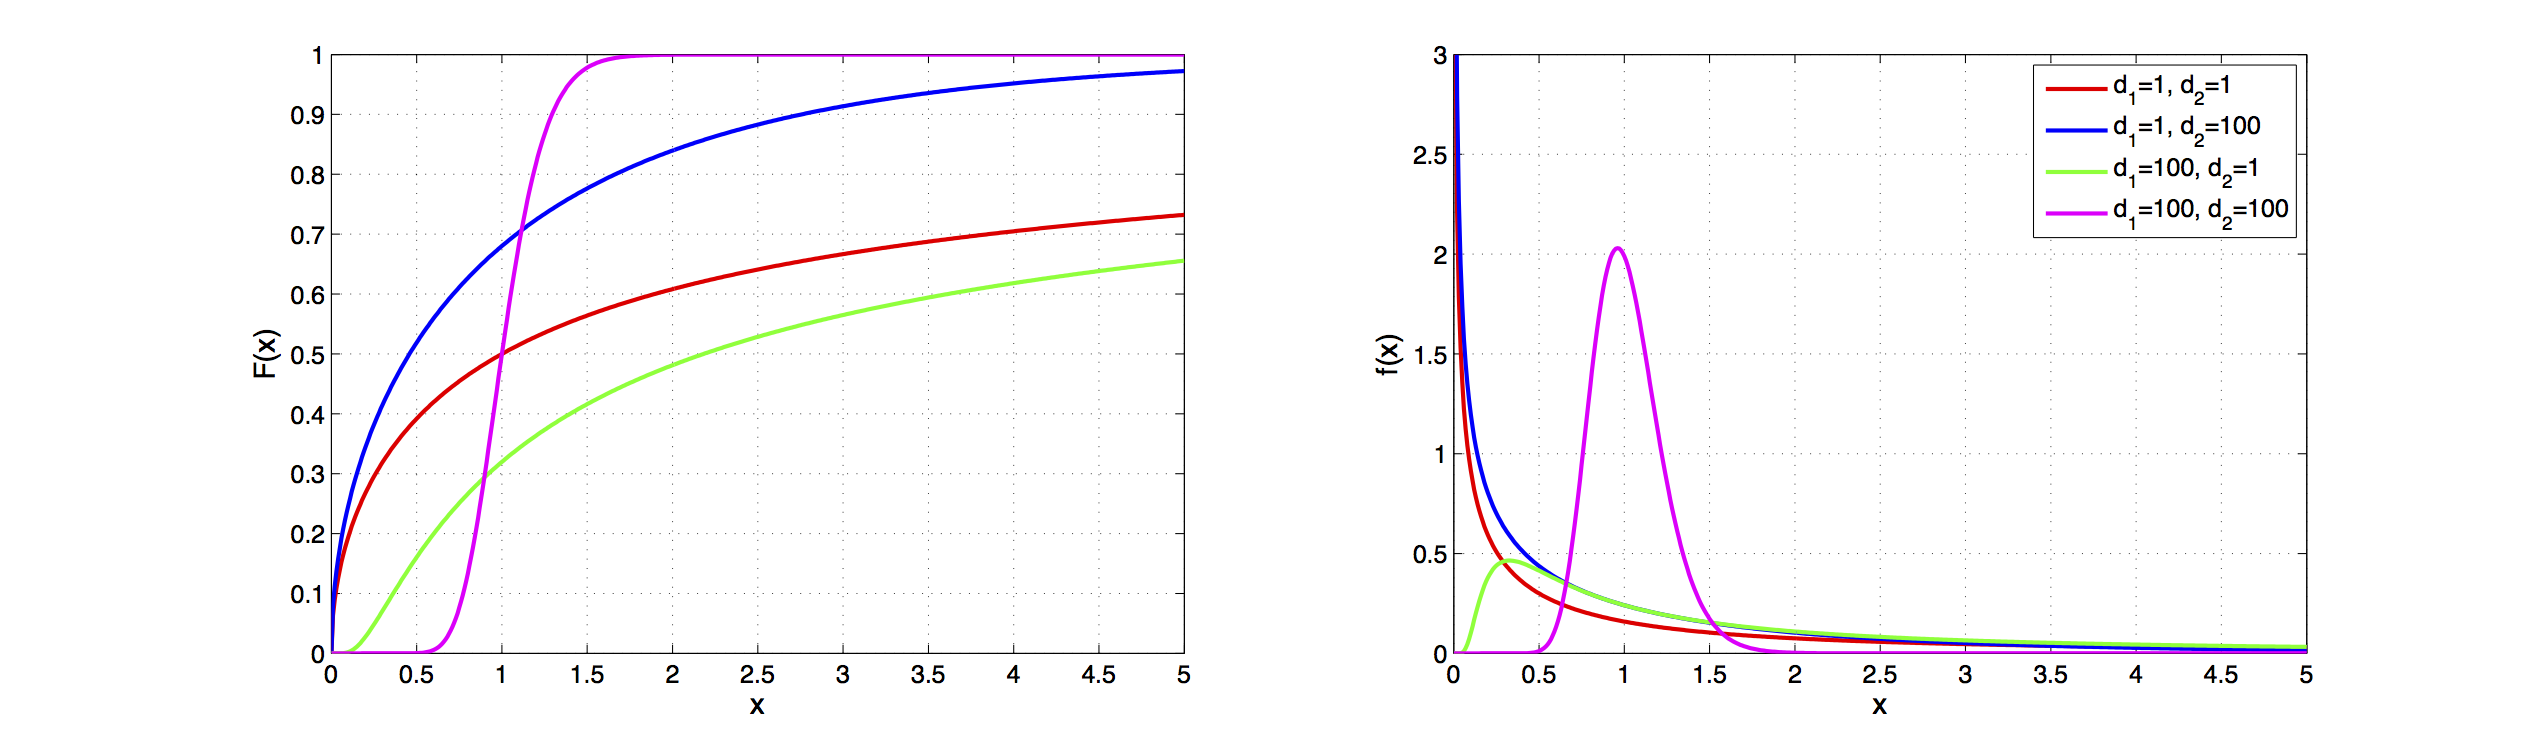
\includegraphics[width=\textwidth]{fish.png}
    \end{center}
     }
\end{frame}

\begin{frame}{Многомерный критерий Грейнджера}
    Зависимость между признаками $x$ и $y$ может оцениваться с учётом возможной зависимости от всех остальных признаков:
    $$y_t = \alpha + \sum_{i=1}^{k_1} \phi_{1i} y_{t-i} + \sum_{i=1}^{k_2} \phi_{2i} x_{t-i} + \sum_{j=1}^m \sum_{i=1}^{k_{j+2}} \phi_{(j+2)i} z^j_{t-i} + \varepsilon_t.$$

    \bigskip

    Для задач с большим количеством признаков могут использоваться регуляризаторы (лассо, ридж).
\end{frame}
 
 
 
\begin{frame}{Граф причинности по Грейнджеру}
	
    \begin{center}
        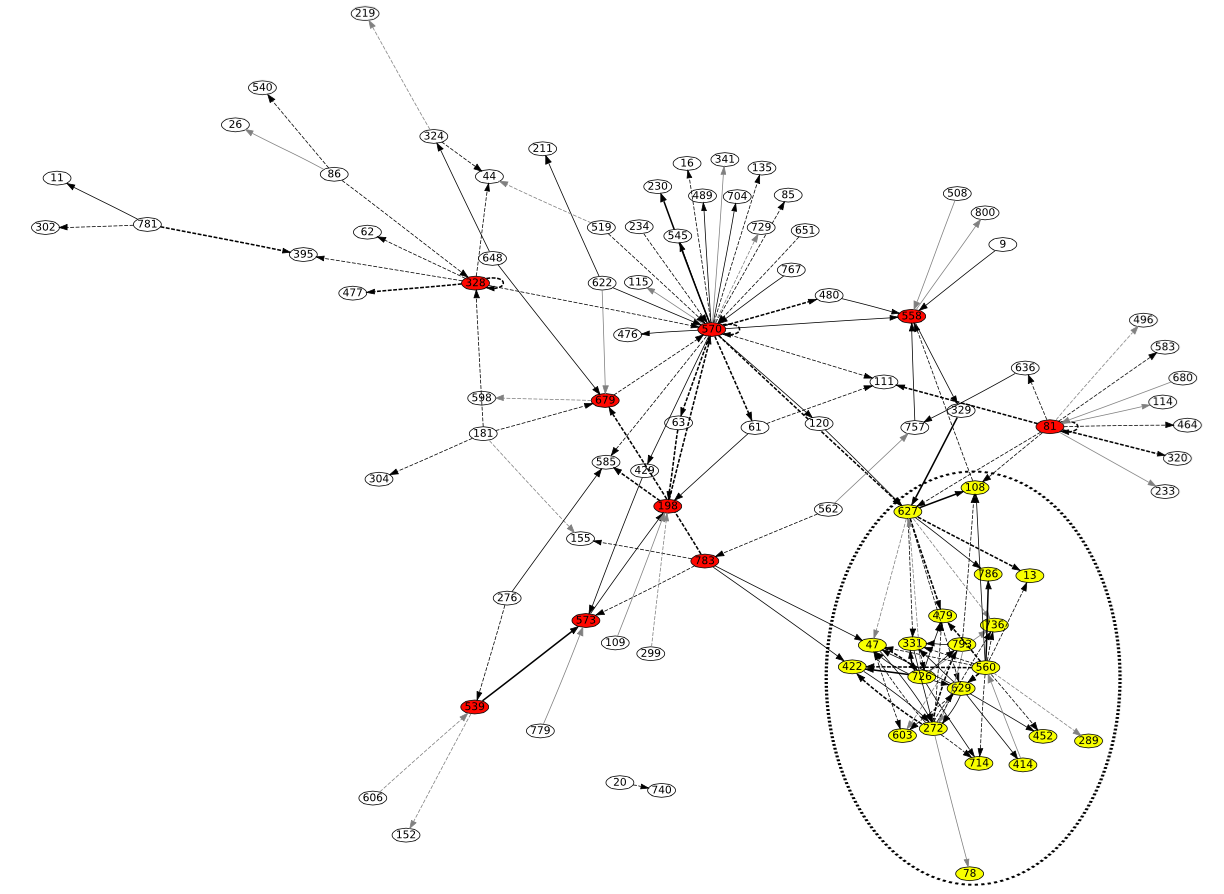
\includegraphics[width=0.7\linewidth]{imgs/granger_graph.eps}
    \end{center}
    Критерий Грейнджера + поправка на множественную проверку гипотез.
\end{frame}



\section{Выводы по графу}
\subsection{Интервенции}
\begin{frame}{Интервенция}
\only<1>{
	$X$ коррелировано с $Y$ $\nRightarrow$ $X$ влияет на $Y$.
	
	Влияние обычно оценивают в эксперименте, когда объектам искусственно назначают разные уровни $X$, но эксперимент можно провести не всегда:
	
	\begin{itemize}
	\item погода $\rightarrow$ лесные пожары — не можем управлять $X$
	\item теленасилие $\rightarrow$ жестокость — тяжело фиксировать уровень $X$ и создать условия для измерения $Y$
	\item потребление алкоголя $\rightarrow$ успеваемость школьников — неэтично
	\end{itemize}
	
	\bigskip
	
	В таких случаях мы вынуждены использовать обзервационные данные, по которым мы хотим оценить эффект \textbf{интервенции}: что будет с $Y$, если мы установим значение $X$ равным $x$? \\
	
	Обозначение: $do(X = x).$	
}
\only<2>{
	\begin{center}
	\begin{tikzpicture}
	    \node at (6,5) (z) {$Z$ (пол)};<br>
	    \node at (4,3) (x) {$X$ (лечение)}; <br>
	    \node at (8,3) (y) {$Y$ (исход)};<br>
	    <br>
	    \path[->] (z) edge (x) ;<br>
	    \path[->] (z) edge (y);<br>
	    \path[->] (x) edge (y) ;<br>
	\end{tikzpicture}
	\end{center}
	
	Оценку эффективности лекарства можно сформулировать в терминах интервенций:
	
	\begin{align*}
	ACE =& \condprob{Y =\text{выздоровление}}{do\left(X = \text{лекарство}\right)} - \\
	    -& \condprob{Y =\text{выздоровление}}{do\left(X = \text{плацебо}\right)}.
	\end{align*}
	
	(average conditional effect).
}
\end{frame}

\begin{frame}{Хирургия графа}
\only<1>{
\textbf{Хирургия графа} — удаление всех ребер, входящих в $X$.\\

\bigskip

Пример 1, исходный граф $G$:
\begin{center}
\begin{tikzpicture}
	\node at (1.5,1.5) (z) {$Z$ (пол)};<br>
	\node at (0,0) (x) {$X$ (лечение)}; <br>
	\node at (3,0) (y) {$Y$ (исход)};<br>
    \path[->] (z) edge (x) ;<br>
    \path[->] (z) edge (y);<br>
    \path[->] (x) edge (y) ;<br>
\end{tikzpicture}
\end{center}
Оперированный граф $G_m$:
\begin{center}
\begin{tikzpicture}   
	    \node at (1.5,1.5) (z) {$Z$ (пол)};<br>
	    \node at (0,0) (x) {$X$ (лечение)}; <br>
	    \node at (3,0) (y) {$Y$ (исход)};<br>
    \path[->] (z) edge (y);<br>
    \path[->] (x) edge (y) ;<br>
\end{tikzpicture}
\end{center}

\bigskip

$\condprob{Y=y}{do\left(X=x\right)} = \mathbf{P}_m\!\left(\left.Y=y\right|X=x\right)$
}
\only<2>{
	В оперированном графе:
	\begin{align*}
	&\mathbf{P}_m\!\left(Z=z\right) = \prob\left(Z=z\right), \\
	&\mathbf{P}_m\!\left(\left.Y=y\right|X=x, Z=z\right) = \condprob{Y=y}{X=x, Z=z}, \\
	\end{align*}
	так как рёбра, входящие в $Z$ и $Y$, не изменились $\Rightarrow$
	
	\begin{align*}
	\condprob{Y =y}{do\left(X = x\right)} &= \mathbf{P}_m\!\left(\left.Y=y\right|X=x\right) = \\
	                                      &= \sum_z \mathbf{P}_m\!\left(\left.Y=y\right|X=x, Z=z\right) \mathbf{P}_m\!\left(Z=z\right) = \\
	                                      &= \sum_z \condprob{Y=y}{X=x, Z=z} \prob\left(Z=z\right).
	\end{align*}
}
\only<3>{
	В примере 1 по полученной формуле:
	
	$\condprob{Y =\text{выздоровление}}{do\left(X = \text{лекарство}\right)} = 0.832$, 
	
	$\condprob{Y =\text{выздоровление}}{do\left(X = \text{плацебо}\right)} = 0.7818$ 
	
	$\Rightarrow$ $ACE = 0.05$.
	
	\bigskip
	
	В примере 2 $G=G_m$:
\begin{center}
\begin{tikzpicture}
	\node at (1.5,1.5) (z) {$Z$ (давление)};<br>
	\node at (0,0) (x) {$X$ (лечение)}; <br>
	\node at (3,0) (y) {$Y$ (исход)};<br>
    \path[->] (x) edge (z) ;<br>
    \path[->] (z) edge (y);<br>
    \path[->] (x) edge (y) ;<br>
\end{tikzpicture}
\end{center}
Значит, 

$\condprob{Y =y}{do\left(X = x\right)} = \mathbf{P}_m\!\left(\left.Y=y\right|X=x\right) = \condprob{Y =y}{X = x}$
	
$\condprob{Y =\text{выздоровление}}{do\left(X = \text{лекарство}\right)} = 0.78$, 
	
$\condprob{Y =\text{выздоровление}}{do\left(X = \text{плацебо}\right)} = 0.83$ 
	
$\Rightarrow$ $ACE = -0.05$.
}
\end{frame}


\begin{frame}{Поправочная формула}
Поправочная формула позволяет вычислить эффект интервенции обуславливанием по вершинам $Z$:
$$\condprob{Y =y}{do\left(X = x\right)} = \sum_z \condprob{Y=y}{X=x, Z=z} \prob\left(Z=z\right).$$
Что это за вершины?

\bigskip

\textbf{Формула причинного эффекта}:
$$\condprob{Y =y}{do\left(X = x\right)} = \sum_z \condprob{Y=y}{X=x, PA=z} \prob\left(PA=z\right),$$
где $PA$~--- родители вершины $X$.
\end{frame}

\subsection{Критерий задней двери}
\begin{frame}{Неизвестные родители}
\begin{center}
\begin{tikzpicture}
	\node at (-1,2) (z) {$U$ (соц.-экон. статус)};<br>
	\node at (0,0) (x) {$X$ (лечение)}; <br>
	\node at (3,2) (w) {$Z$ (вес)};<br>	
	\node at (3,0) (y) {$Y$ (исход)};<br>
    \path[->] (z) edge (w) ;<br>
    \path[->] (z) edge (x);<br>
    \path[->] (x) edge (y) ;<br>
    \path[->] (w) edge (y) ;<br>
\end{tikzpicture}
\end{center}

Социоэкономический статус — ненаблюдаемая величина; как оценить эффект интервенции по $X$?
\end{frame}

\begin{frame}{Критерий задней двери (KЗД)}
\only<1>{
Для упорядоченной пары вершин $(X,Y)$ в ациклическом графе $G$ множество вершин $Z$ удовлетворяет \textbf{критерию задней двери}, если:
\begin{itemize}
\item $Z$ не содержит потомков $X$
\item $Z$ блокирует все пути между $X$ и $Y$, содержащие $X\leftarrow$.
\end{itemize}

\bigskip

Если $Z$ удовлетворяет КЗД для $(X,Y)$, то 
$$\condprob{Y =y}{do\left(X = x\right)} = \sum_z \condprob{Y=y}{X=x, Z=z} \prob\left(Z=z\right)$$
(формула задней двери).
}
\only<2>{
Чтобы вычислять меньше условных вероятностей, ФЗД можно упростить:
\begin{align*}
\condprob{Y =y}{do\left(X = x\right)} &= \sum_z \condprob{Y=y}{X=x, Z=z} \prob\left(Z=z\right) = \\
&= \sum_z\frac{\prob\left(X=x, Y=y, Z=z\right)}{\condprob{X=x}{Z=z}}
\end{align*}
В таком виде 
\begin{itemize}
	\item метод называется \textbf{обратное вероятностное взвешивание}
	\item знаменатель $\condprob{X=x}{Z=z}$~--- propensity score. 
\end{itemize}

}
\end{frame}

\subsection{Критерий передней двери}
\begin{frame}{Неизвестные родители}
Вызывает ли курение рак?
\begin{center}
	\begin{tikzpicture}
	\node at (2,2) (u) {$U$ (генотип)};<br>
	\node at (0,0) (x) {$X$ (курение)}; <br>
	\node at (4,0) (y) {$Y$ (рак)};<br>
	\path[->] (u) edge (x) ;<br>
	\path[->] (x) edge (y);<br>
	\path[->] (u) edge (y) ;<br>
	\end{tikzpicture}
\end{center}

\bigskip

\begin{tabular}{|p{2cm}|p{2cm}|p{2cm}|c}
	\cline{1-3}
	$\Sigma$ & курильщики & некурящие & \\
	\cline{1-3} 
	нет рака & 341 & 59   & курильщики болеют \\
	\cline{1-3}
	есть рак & 39  & 361  & на 75.25\% реже \\
	\cline{1-3}
	& 15\% & 90.25\% & \\
	\cline{1-3}
\end{tabular} \\





\end{frame}

\begin{frame}{Курение}
\only<1>{
%\begin{tabular}{|c|c|c|}\hline 
%	$\Sigma$ & курильщики & некурящие \\ \hline 
%	нет рака & 341        & 59 \\ \hline 
%	есть рак & 39         & 361 \\ \hline 
%	         & 15\%       & 90.25\% \\ \hline 
%\end{tabular} \\
%$ $ \\
%$ $ \\
%\begin{tabular}{|c|c|c|}\hline 
%	смола    & курильщики & некурящие \\ \hline 
%	нет рака & 323        & 1 \\ \hline 
%	есть рак & 57         & 19 \\ \hline 
%	         & 15\%       & 95\% \\ \hline 
%\end{tabular} \\
%$ $ \\
%$ $ \\
%\begin{tabular}{|c|c|c|}\hline 
%	нет смолы & курильщики & некурящие \\ \hline 
%	нет рака  & 18         & 38 \\ \hline 
%	есть рак  & 2          & 342 \\ \hline 
%	          & 10\%       & 90\% \\ \hline 
%\end{tabular}
%

\begin{center}
	\begin{tikzpicture}
	\node at (2,2) (u) {$U$ (генотип)};<br>
	\node at (2.15,0) (z) {$Z$ (смола)};<br>
	\node at (0,0) (x) {$X$ (курение)}; <br>
	\node at (4,0) (y) {$Y$ (рак)};<br>
	\path[->] (u) edge (x) ;<br>
	\path[->] (x) edge (z);<br>
	\path[->] (z) edge (y) ;<br>
	\path[->] (u) edge (y) ;<br>
	\end{tikzpicture}
\end{center}

%\begin{tabular}{|p{2cm}|p{2cm}|p{2cm}|c}
%	\cline{1-3}
%	$\Sigma$ & курильщики & некурящие & \\
%	\cline{1-3} 
%	нет рака & 341 & 59   & курильщики болеют \\
%	\cline{1-3}
%    есть рак & 39  & 361  & на 75.25\% реже \\
%	\cline{1-3}
%	         & 15\% & 90.25\% & \\
%	\cline{1-3}
%\end{tabular} \\
%$ $ \\
%$ $ \\

\bigskip

  \begin{tabular}{|p{2cm}|p{2cm}|p{2cm}|c}
	\cline{1-3}
    \textbf{смола} & курильщики & некурящие &\\
	\cline{1-3}
	нет рака & 323        & 1 & курильщики болеют \\
	\cline{1-3}
	есть рак & 57         & 19 &  на 80\% реже \\
	\cline{1-3}
	 & 15\%       & 95\% & \\
	\cline{1-3}
\end{tabular} \\
$ $ \\
$ $ \\
  \begin{tabular}{|p{2cm}|p{2cm}|p{2cm}|c}
	\cline{1-3}
	\textbf{нет смолы} & курильщики & некурящие & \\
	\cline{1-3}
	нет рака  & 18         & 38 & курильщики болеют \\
	\cline{1-3}
    есть рак  & 2          & 342 & на 80\% реже \\
	\cline{1-3}
	 & 10\%       & 90\% \\
	\cline{1-3}
\end{tabular}

\bigskip

Курить полезно?
}
\only<2>{
У курильщиков смола в 95\% случаев вместо 5\%; у курильщиков смола увеличивает риск рака с 10\% до 15\%; у некурящих~--- с 90\% до 95\%.

Курить вредно?

\bigskip

Поможет граф!
}
\only<3>{
Поправочная формула (КЗД для пустого множества и для $ X $):

\begin{align*}
&\condprob{Z=z}{do\left(X=x\right)} = \condprob{Z=z}{X=x}, \\
&\condprob{Y=y}{do\left(Z=z\right)} = \sum_{x'}\condprob{Y=y}{Z=z, X=x'} \prob\left(X=x'\right) \\
\end{align*}

\begin{center}
	\begin{tikzpicture}
	\node at (2,1) (u) {$U$ (генотип)};<br>
	\node at (2.15,0) (z) {$Z$ (смола)};<br>
	\node at (0,0) (x) {$X$ (курение)}; <br>
	\node at (4,0) (y) {$Y$ (рак)};<br>
	\path[->] (u) edge (x) ;<br>
	\path[->] (x) edge (z);<br>
	\path[->] (z) edge (y) ;<br>
	\path[->] (u) edge (y) ;<br>
	\end{tikzpicture}
\end{center}

\begin{align*}
&\condprob{Y=y}{do\left(X=x\right)} = \\
&= \sum_z \condprob{Y=y}{do\left(Z=z\right)} \condprob{Z=z}{do\left(X=x\right)} =  \\
&= \sum_z \sum_{x'}\condprob{Y=y}{Z=z, X=x'} \condprob{Z=z}{X=x}\prob\left(X=x'\right). \\
\end{align*}
}
\end{frame}

\begin{frame}{Критерий передней двери (КПД)}
Для упорядоченной пары вершин $(X,Y)$ в ациклическом графе $G$ множество вершин $Z$ удовлетворяет \textbf{критерию передней двери}, если:
\begin{itemize}
\item $Z$ перекрывает все направленные пути из $X$ в $Y$
\item нет незакрытых путей через заднюю дверь из $X$ в $Z$
\item все пути через заднюю дверь из $Z$ в $Y$ блокируются $X$
\end{itemize}

\bigskip

Если $Z$ удовлетворяет КПД для $(X,Y)$, то 
\begin{align*}
&\condprob{Y =y}{do\left(X = x\right)} = \\
&=\sum_z \condprob{Z=z}{X=x}\sum_{x'} \condprob{Y=y}{X=x', Z=z}  \prob\left(X=x'\right)
\end{align*}
(формула передней двери).
\end{frame}

\section{}
\begin{frame}{Литература}
    \begin{itemize}
    \item причинные графы и выводы по ним~--- Pearl
    \item восстановление графов по статическим данным~--- Nagarajan, глава 2
	\item причинность по Грейнджеру~--- Kirchgassner, глава~3
    \end{itemize}

	\bigskip
   
	Kirchgassner G., Wolters J., Hassler U. {\em Introduction to modern time series analysis}, 2013.
	
	\bigskip
			
	Nagarajan R., Scutari M., Lebre S. {\em Bayesian Networks in R with Applications in Systems Biology}, 2013. 
	
	\bigskip
			
	Pearl J., Glymour M., Jewell N.P. \em{Causal Inference in Statistics: A Primer}, 2016.
\end{frame}

\iffalse
\begin{frame}{Python}
    \textbf{Требуемые библиотеки:}\\
    \begin{itemize}
    \item networkx\textcolor{gray}{ ==2.3} --- работа с графами;
    \item causalgraphicalmodels\textcolor{gray}{==0.0.4} --- причинность;
    \item causality\textcolor{gray}{==0.0.9} --- причинность;
    \end{itemize}
    \bf{Установка пакетов:}\\
    \begin{itemize}
    
    \item \tt{[sudo] pip install [package name]}
    \item \tt{[sudo] conda install [package name]}

    \end{itemize}
\end{frame}
\begin{frame}{Лаба 2}
\begin{itemize}
\item 4 простых задания;
\item 3 задания ``посложнее'';
\item дедлайн: 1 неделя.
\end{itemize}
\end{frame}

\begin{frame}{Задание 1}
\begin{block}{}
Сравнить МНК-оценку для линейной регрессии с методом наименьших модулей в случае, когда шум порожден из распределения Лапласа.
Когда оценки совпадают, а когда сильно различаются? 
\end{block}
\end{frame}

\begin{frame}{Задание 2}
\begin{block}{}
Проверить адекватность модели и доверительных интервалов модели линейной регрессии для выборки с гедеростичной ошибок.
\end{block}
\end{frame}


\begin{frame}{Задание 3}
\begin{block}{}
Проверить мощность и консервативность критериев Вальда и Фишера для линейной модели.
\end{block}
\end{frame}


\begin{frame}{Задание 4}
\begin{block}{}
Изучить поведение модели пуассоновской регрессии для overdispersed-выборок.
\end{block}
\end{frame}

\begin{frame}{Задание 5}
\begin{block}{}
Задано изображение и набор признаков, соответствующий каждому пикселю.
Требуется восстановить отображение из признакового пространства в пространство изображений, а также проинтерпретировать основные признаки. 
\end{block}
\end{frame}


\begin{frame}{Задание 6}
\begin{block}{}
Задан набор записей речи людей и информация по ним (возраст, пол, страна, родной язык). Возьмем в качестве интегрального признака речи zero-crossing.
Требуется изучить зависимость zero-crossing от факторов возраста, пола, родного языка.
\end{block}

\end{frame}

\begin{frame}{Задание 7}
\begin{block}{}
Задана выборка с стеганографическими изображениями  (1\%) и шумными изображениями (99\%, шум из распределения Лапласа). 
Стеганографические изображения генерируются следующим образом:
\begin{enumerate}
\item каждая буква английского слова конвертируется в число от 0 до 25 (по алфавитному порядку);
\item полученный вектор домножается на неизвестный коэффициент $\alpha$ и складывается с gray-scale-значениями изображения;
\end{enumerate}

Обучающая выборка: набор исходных изображений, измененных изображений и скрытых слов.

Требуется найти $\alpha$ и раскодировать контрольное изображение.
\end{block}
\end{frame}


\fi
\end{document}
